\chapter{Implementation}
\label{chapter:implementation}

In chapter 3, it was presented an overview of the SmartLighting project, giving an outline of the requirements and use cases. Also, to satisfy the project needs, an overview of the several scenarios of functioning as well as a possible architecture for the system was presented.

The objective for this chapter is to describe the steps and decisions taken, and the reasoning behind the implemented features. It starts in section \ref{implementation:objectives}, by presenting the objectives for the implementation, following by the used technologies on the several components in section \ref{implementation:technologies}. After that, in sections \ref{implementation:devices} and \ref{implementation:rules}, it is presented the standards used to access the devices and to define rules, respectively. Following, in section \ref{implementation:architecture}, the whole system's architecture as well as the functioning of its components is described. 

Since one of the requirements and objectives for this project was the existence of failure handling mechanisms, in section \ref{implementation:scenarios}, it is described the implementation taking into account the several scenarios addressed in the previous chapter. 

\newpage

\section{Objectives}
\label{implementation:objectives}

Although the implementation of the whole solution, presented in chapter \ref{chapter:architecture}, would be optimal to validate the project, it would be unrealistic due to the amount of time necessary to do so and the limited time available for this dissertation. Since some of the features were already implemented, such as a working platform to create and manage rules, a \ac{cep} engine and a simple gateway to communicate with devices through BLE, this dissertation's main focus was in the implementation of gateways capable of implement automation rules, alike to the ones implemented by the CEP engine, as well as give them means to adapt to failing and emergency states. For that reason, was also implemented a gateway manager to act as a monitor for the gateways, being able to control not only the functioning of each one of them as well as manage the distribution of rules and devices throughout the gateways.

Looking at the architecture presented in chapter 3, the component for the user management dashboard was not implemented for the scope of this work. Apart from this, all the features mentioned were implemented and are detailed in the continuation of this chapter.



\section{Adopted  Technologies}
\label{implementation:technologies}

This section aims to discuss the technologies chosen for the different components of the architecture. This choices will be explained taking into account the requirements for this project, however, it is important to note that there are no perfect solutions and, in some cases, several approaches could have been taken.

Since there was a dissertation that already implemented some features like the \ac{cep} engine and the \ac{bm}, some of the technologies used in this dissertation were influenced by past decisions. As far as the \ac{cep} engine concerns, the choice was the WSO2 \ac{cep} \cite{wso2}, since its features addressed all requirements, that such system would need, to fit this project's requirements. For the purpose of this dissertation both the \ac{cep} engine and the \ac{bm} as well as the communication between them, did not affect any of the new implemented features, however, since MQTT was primarily used as the elect protocol for communications in the referred dissertation, the implemented features presented in this work followed the same path.

Finally, it is important to state that the standard used, in SmartLighting project, for both object definition to read and write information to/from devices, and the rules structure, were also maintained and will be described in the following sections. 

\section{Access to Devices}
\label{implementation:devices}

Devices like sensors, which measure environment changes, and actuators, that trigger mechanisms to make changes in that same environment, are fundamental pieces to implement a smart and automated environment. Since there are a huge variety of devices with different characteristics, in order to enable extensibility for the system, the access to those devices, as well as the messages format, should be standardised. In another dissertation for this project, a standard following the IP Smart Objects Alliance guidelines was made and is illustrated in Figure \ref{fig:obj}

\begin{figure}[H]
	\centering
	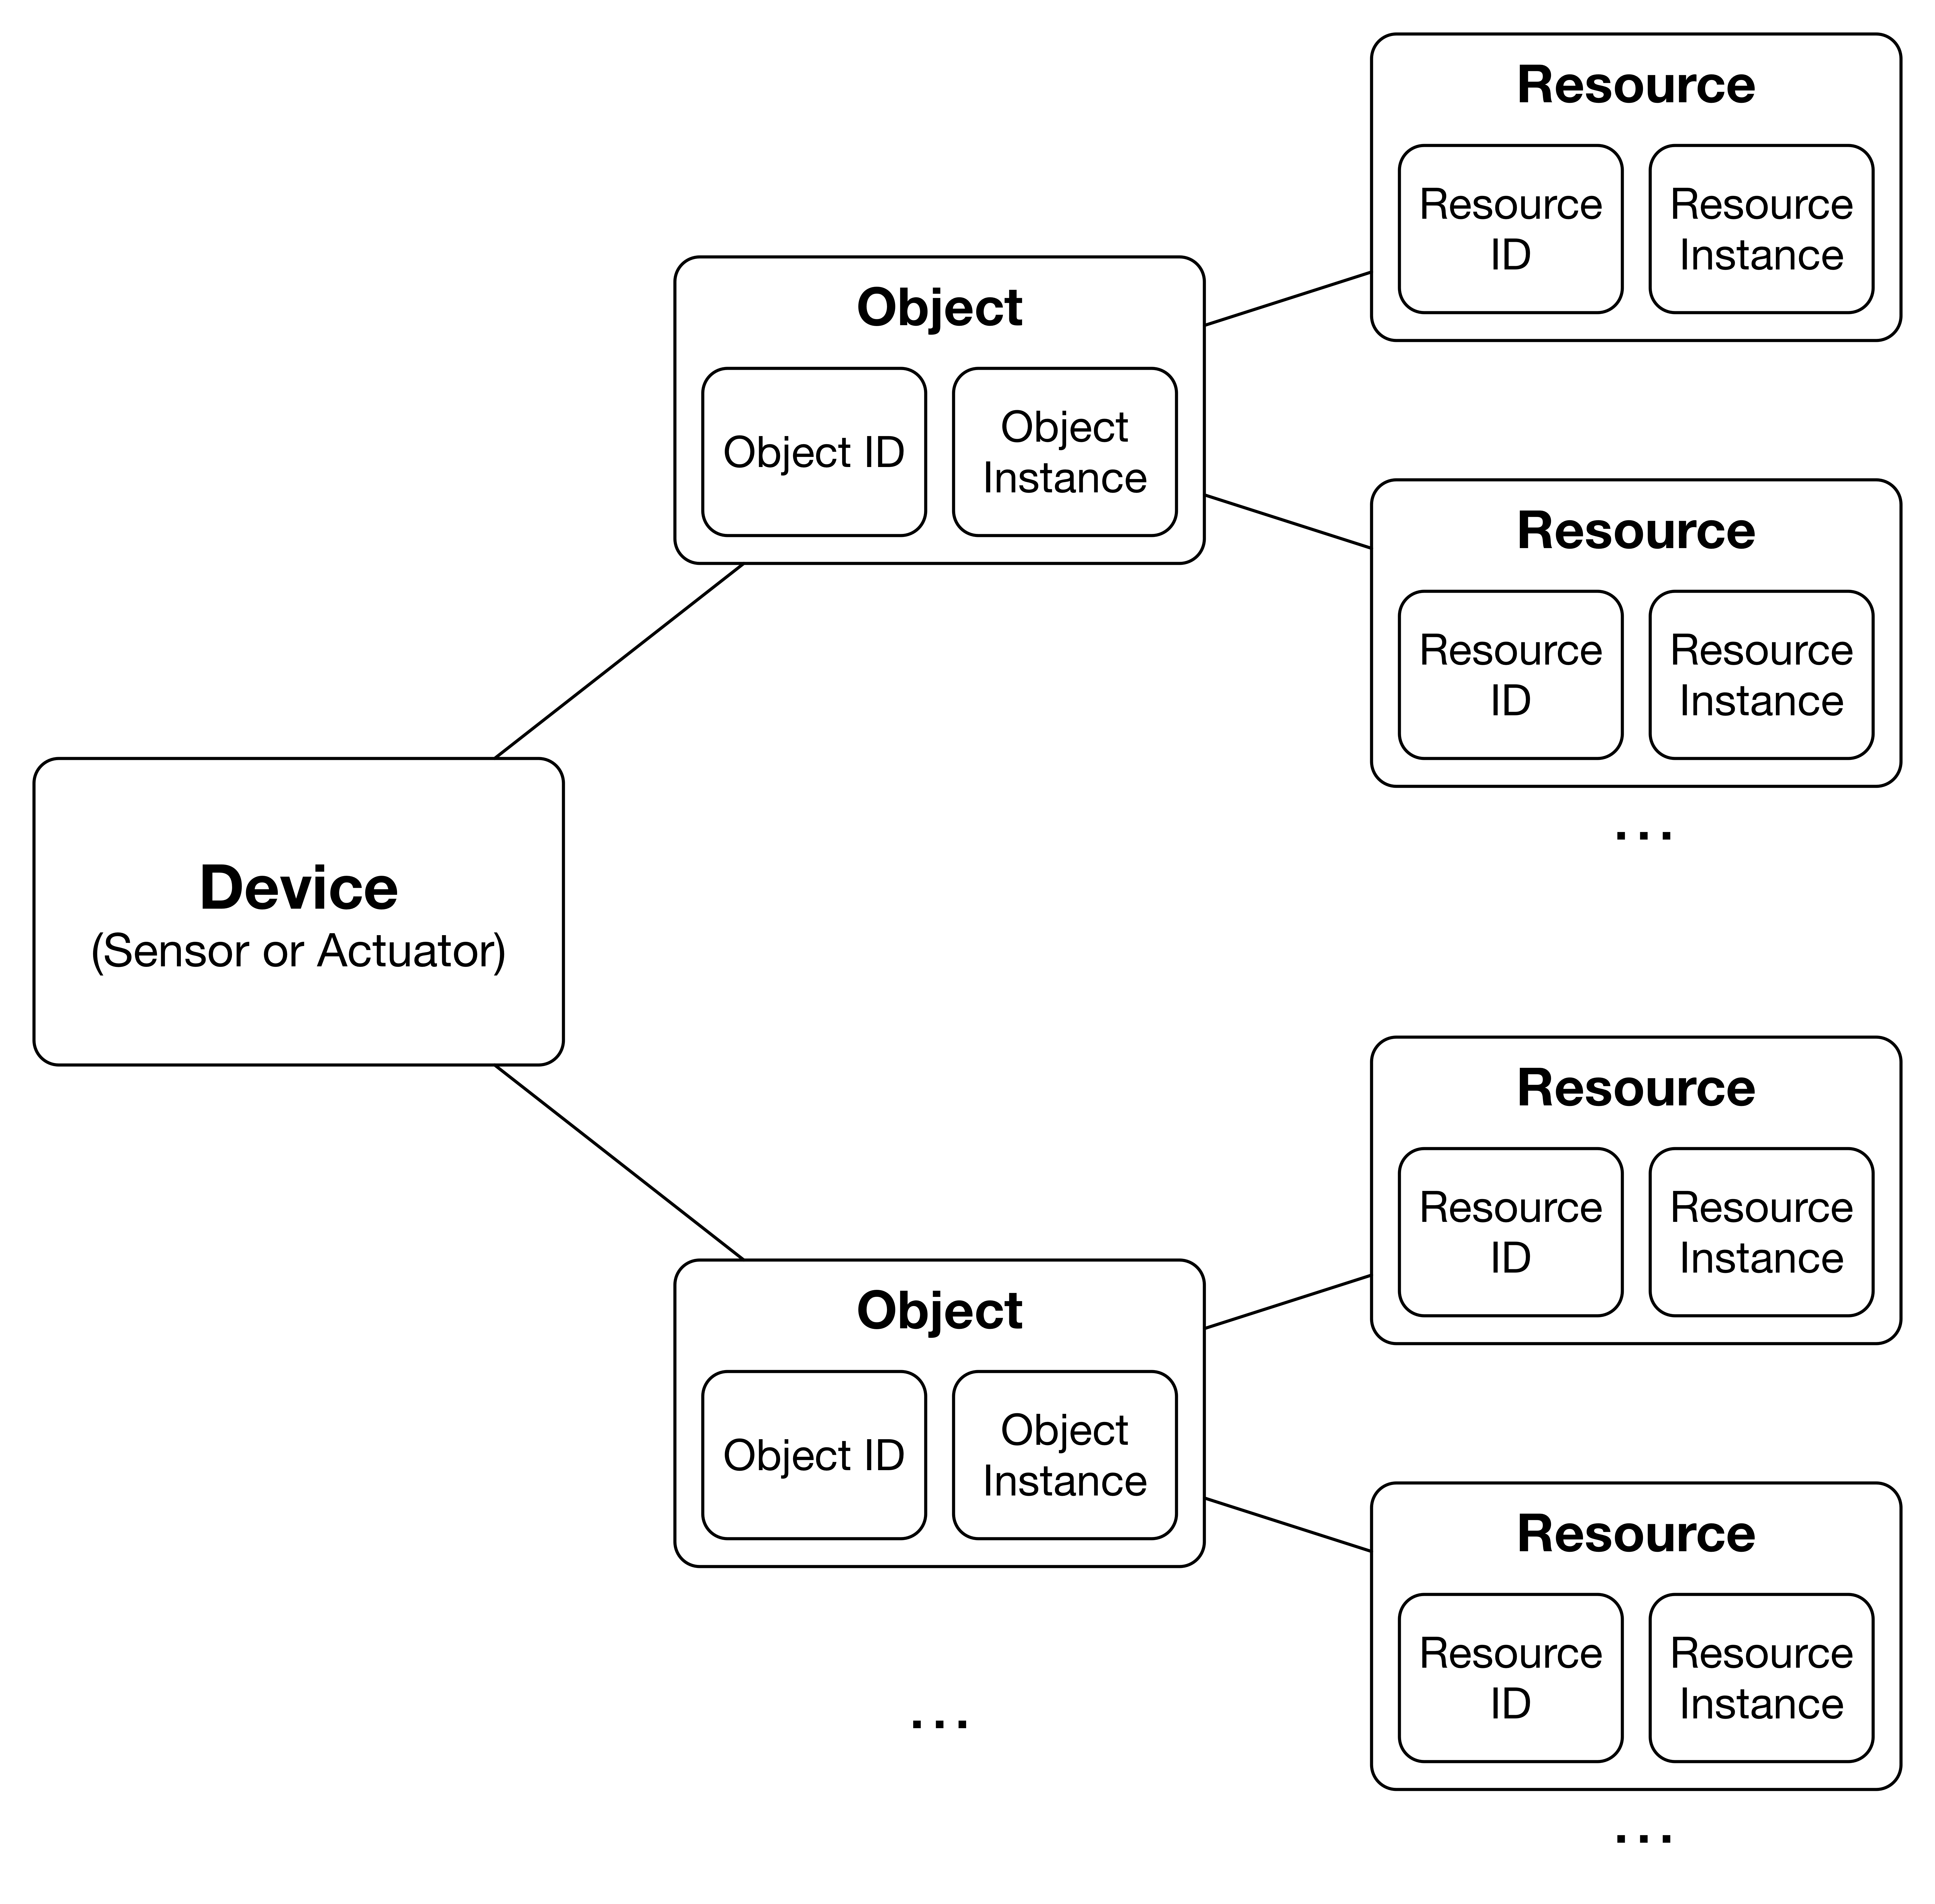
\includegraphics[width=0.9\textwidth]{figures/obj.png}
	\caption{Device objects representation}
	\label{fig:obj}
\end{figure}

In this representation, a device can have multiple objects (sensors and/or actuators), identified through an ID and an object instance. Per example, a device can have multiple sensing or actuating capabilities, each one of them identified with a different ID. A device with two motion sensors, will have two objects with the same ID but different object instances. 

Inside the representation of each object, the information is divided in resources. Resources represent the available features that each object provides, such as the available values that can be read or written, or the actions that can be triggered. As an example, an luminaire actuator object can have resources to read the current state of the luminaire, turn  on/off or dim the light to a certain value, each one of them represented with a different ID. The resource instance is used when, per example, when an actuator for aluminaire with two lamps offers the same resources for each lamp separately.

Using this representation, the properties of a device can me accessed using an Uniform Resource Identifier (URI) the following way: 


\begin{minted}[
frame=single
]{nginx}

.../Object_ID/Object_Instance/Resource_ID/Resource_Instance
	

\end{minted}
	
For instance, a device with a temperature sensor that offers the possibility of check the current state or check the minimum value measured by the sensor since it is ON, can be illustrated and accessed the following way:


\begin{figure}[H]
	\centering
	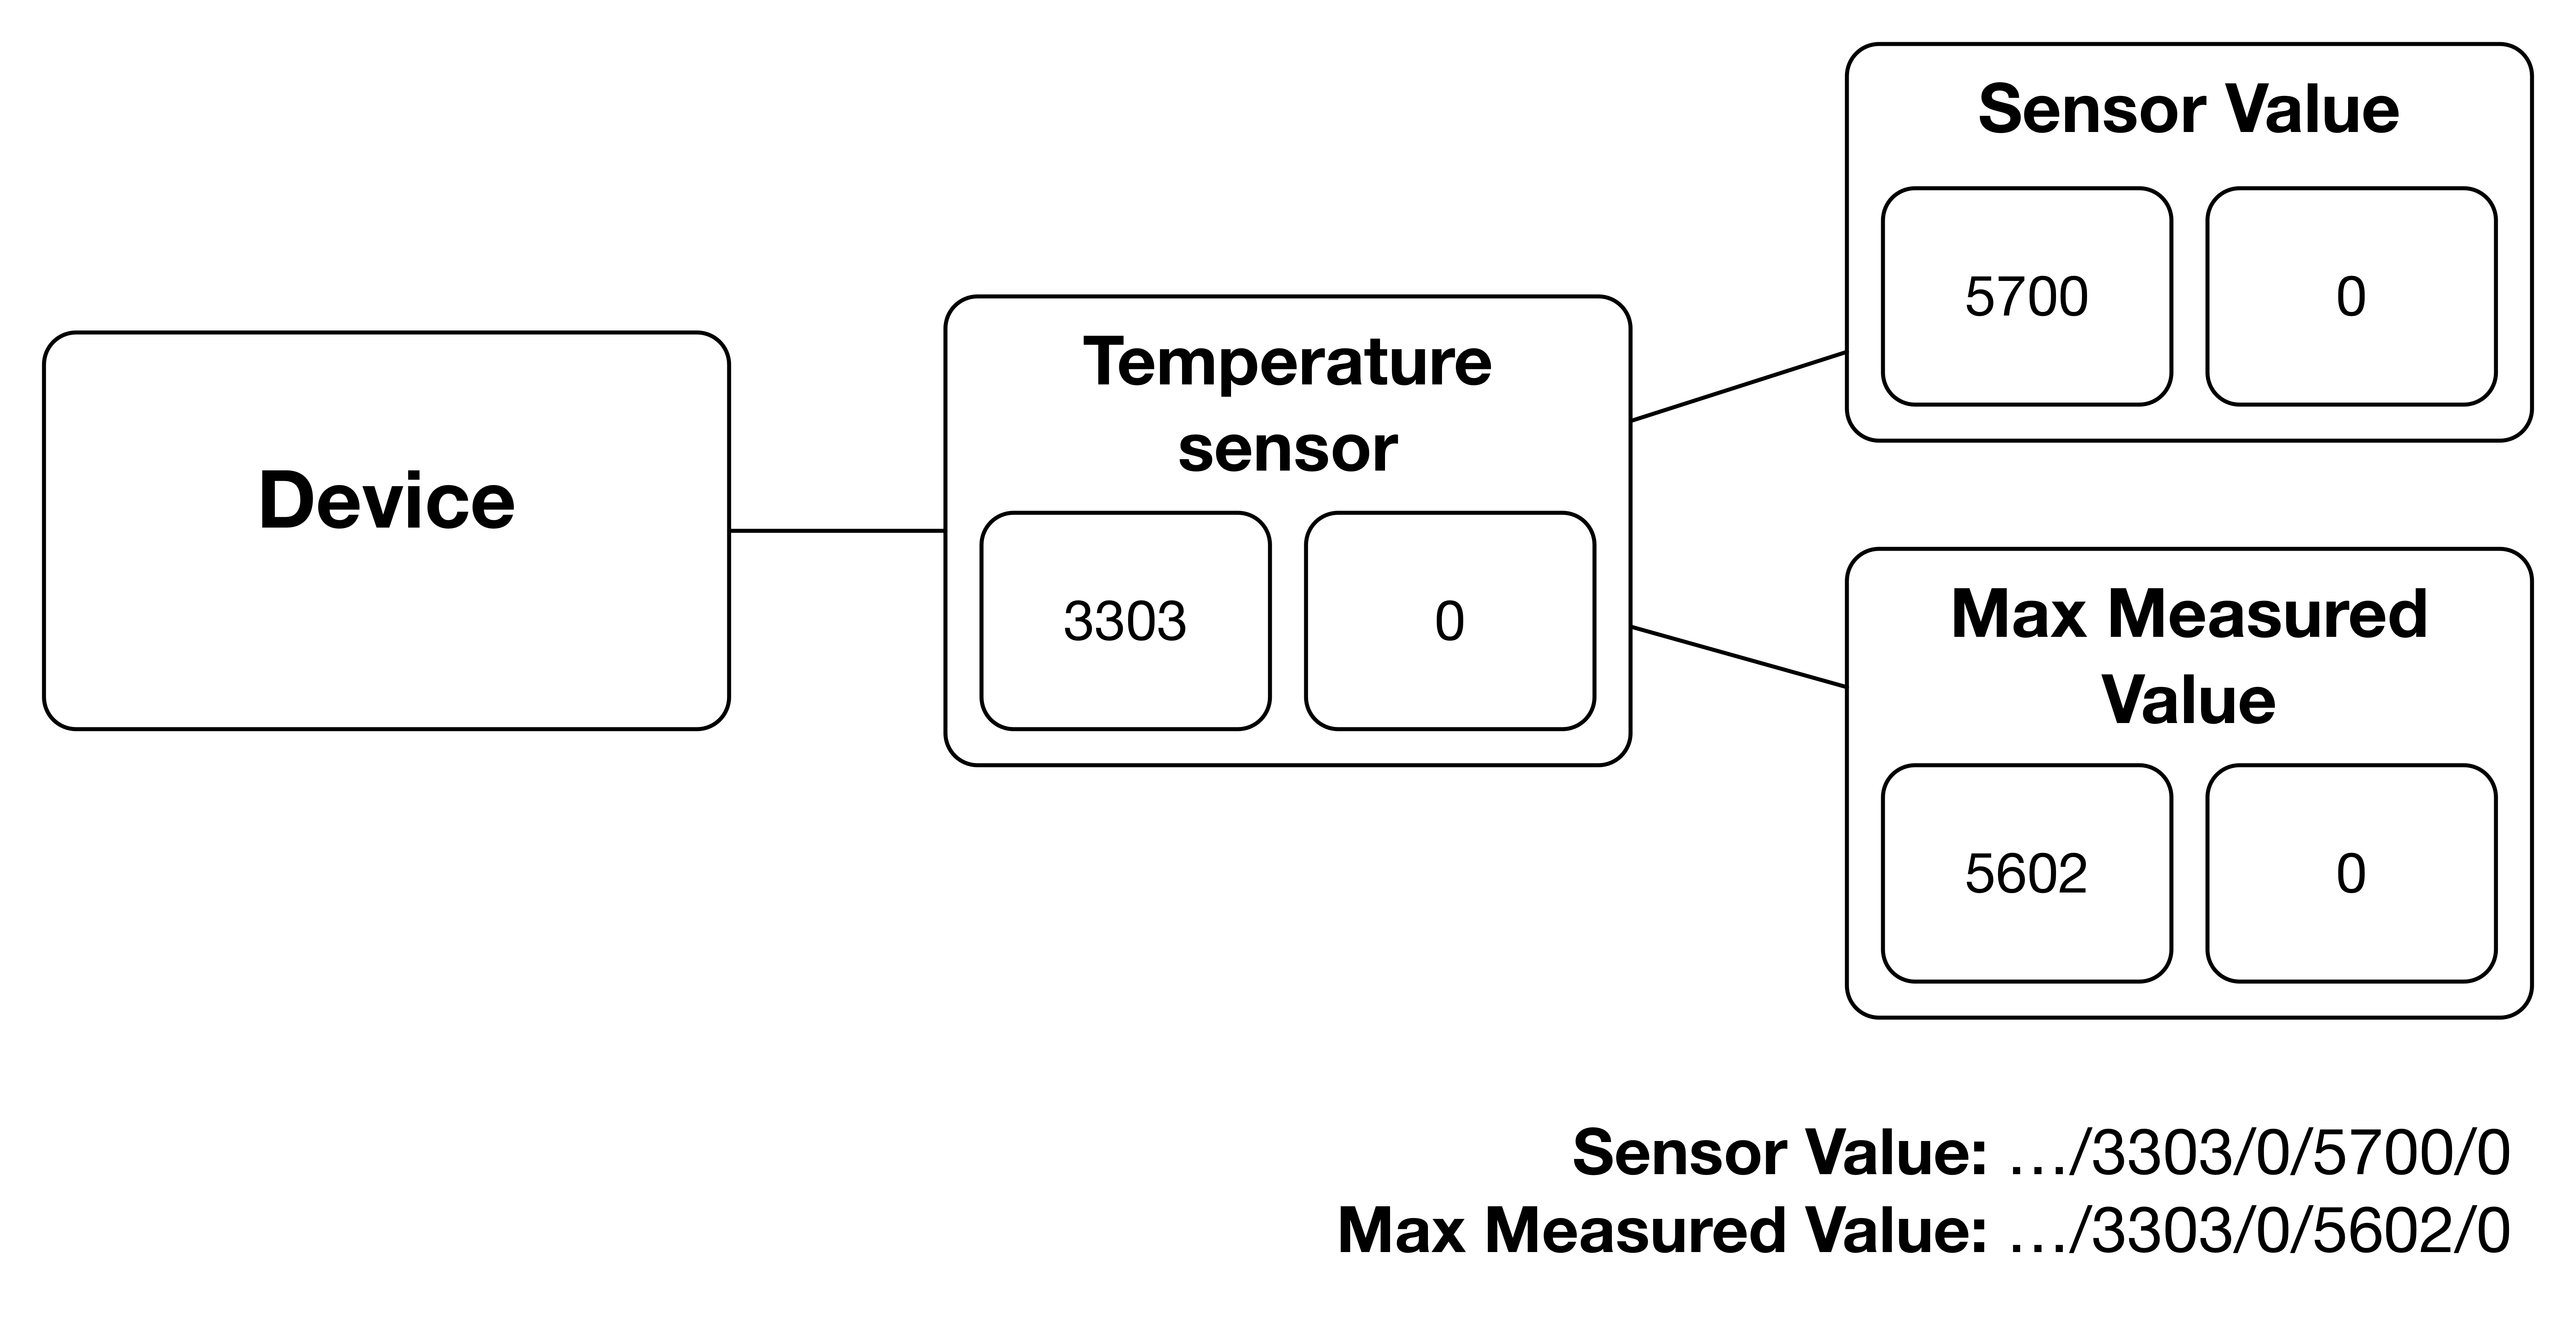
\includegraphics[width=0.9\textwidth]{figures/obj2.png}
	\caption{Access to a device resources.}
	\label{fig:obj2}
\end{figure}
	
Since the protocol used for this project was \ac{mqtt}, which allows to subscribe and publish messages in specific topics, this URI can be used in the topic to address each device resource. 

As stated before, due to the work done in other dissertation for this project, the message format to communicate with devices was chosen based on the event format supported by the WSO2 \ac{cep}, chosen as the \ac{cep} engine for this project. The format is represented in Snippet \ref{snippet:example}.

\begin{listing}[H]
\begin{minted}[
frame=single
]{json}

{
    "event": {
        "metaData": { 
            "attribute_1": ***,
            "attribute_2": ***,
            ...
        },
        "correlationData": {
            "attribute_1": ***,
            "attribute_2": ***,
            ...
        }, 
        "payloadData": {
            "attribute_1": ***, 
            "attribute_2": ***,
        }
    }
}


\end{minted}
\caption{Example of a simplified message for an event sent to a device.}
\label{snippet:example}
\end{listing}

This event messages are divided in three main logical sections: Payload Data, Correlation Data and Meta Data. Payload Data is the most important data to be transported, such as, the values that are sent to and from devices. The Correlation Data transports information that allows correlating events and lastly, the Meta Data is where other attributes that describe the event can be included. In Snippet \ref{snippet:todevice} is represented an example message of an event sent to a device.

\begin{listing}[H]
\begin{minted}[
frame=single
]{json}
{
    "event": {
        "metaData": {
            "operation":"set"
        }, 
        "payloadData": {
            "value": 15 
        }
    } 
}

\end{minted}
\caption{Example of a simplified message for an event sent to a device.}
\label{snippet:todevice}
\end{listing}

This message would set the value 15 on a device's resource if sent to the corresponding topic using the format presented above.
	
\section{Architecture}
\label{implementation:architecture}
Taking into consideration the objectives and adopted technologies addressed in chapters \ref{implementation:objectives} and \ref{implementation:technologies}, the implemented architecture is represented in Figure \ref{fig:arch2}. Comparing this architecture to the one presented in Figure \ref{fig:arch}, it is clear the use of MQTT as the main communication protocol, the removal of the User Management component, since it was not in the scope for this dissertation, and as far as the \ac{cep} engine and the Building Manager concerns, those components were already implemented, as stated before. The BLE Adapter which is part of the gateway was also already implemented. Lastly, the MQTT broker used in this implementation was Mosquitto\footnote{https://mosquitto.org/}, which is a lightweight broker suited for \ac{iot} environments which implements the latest versions on MQTT protocol . 

For the scope of this dissertation, the focus was the implementation of a Gateway with automation capabilities, and also a Gateway Manager to handle not only the rule and device distribution between the available gateways, but also to handling fails in order to maintain the system working even in emergency states.


\begin{figure}[H]
	\centering
	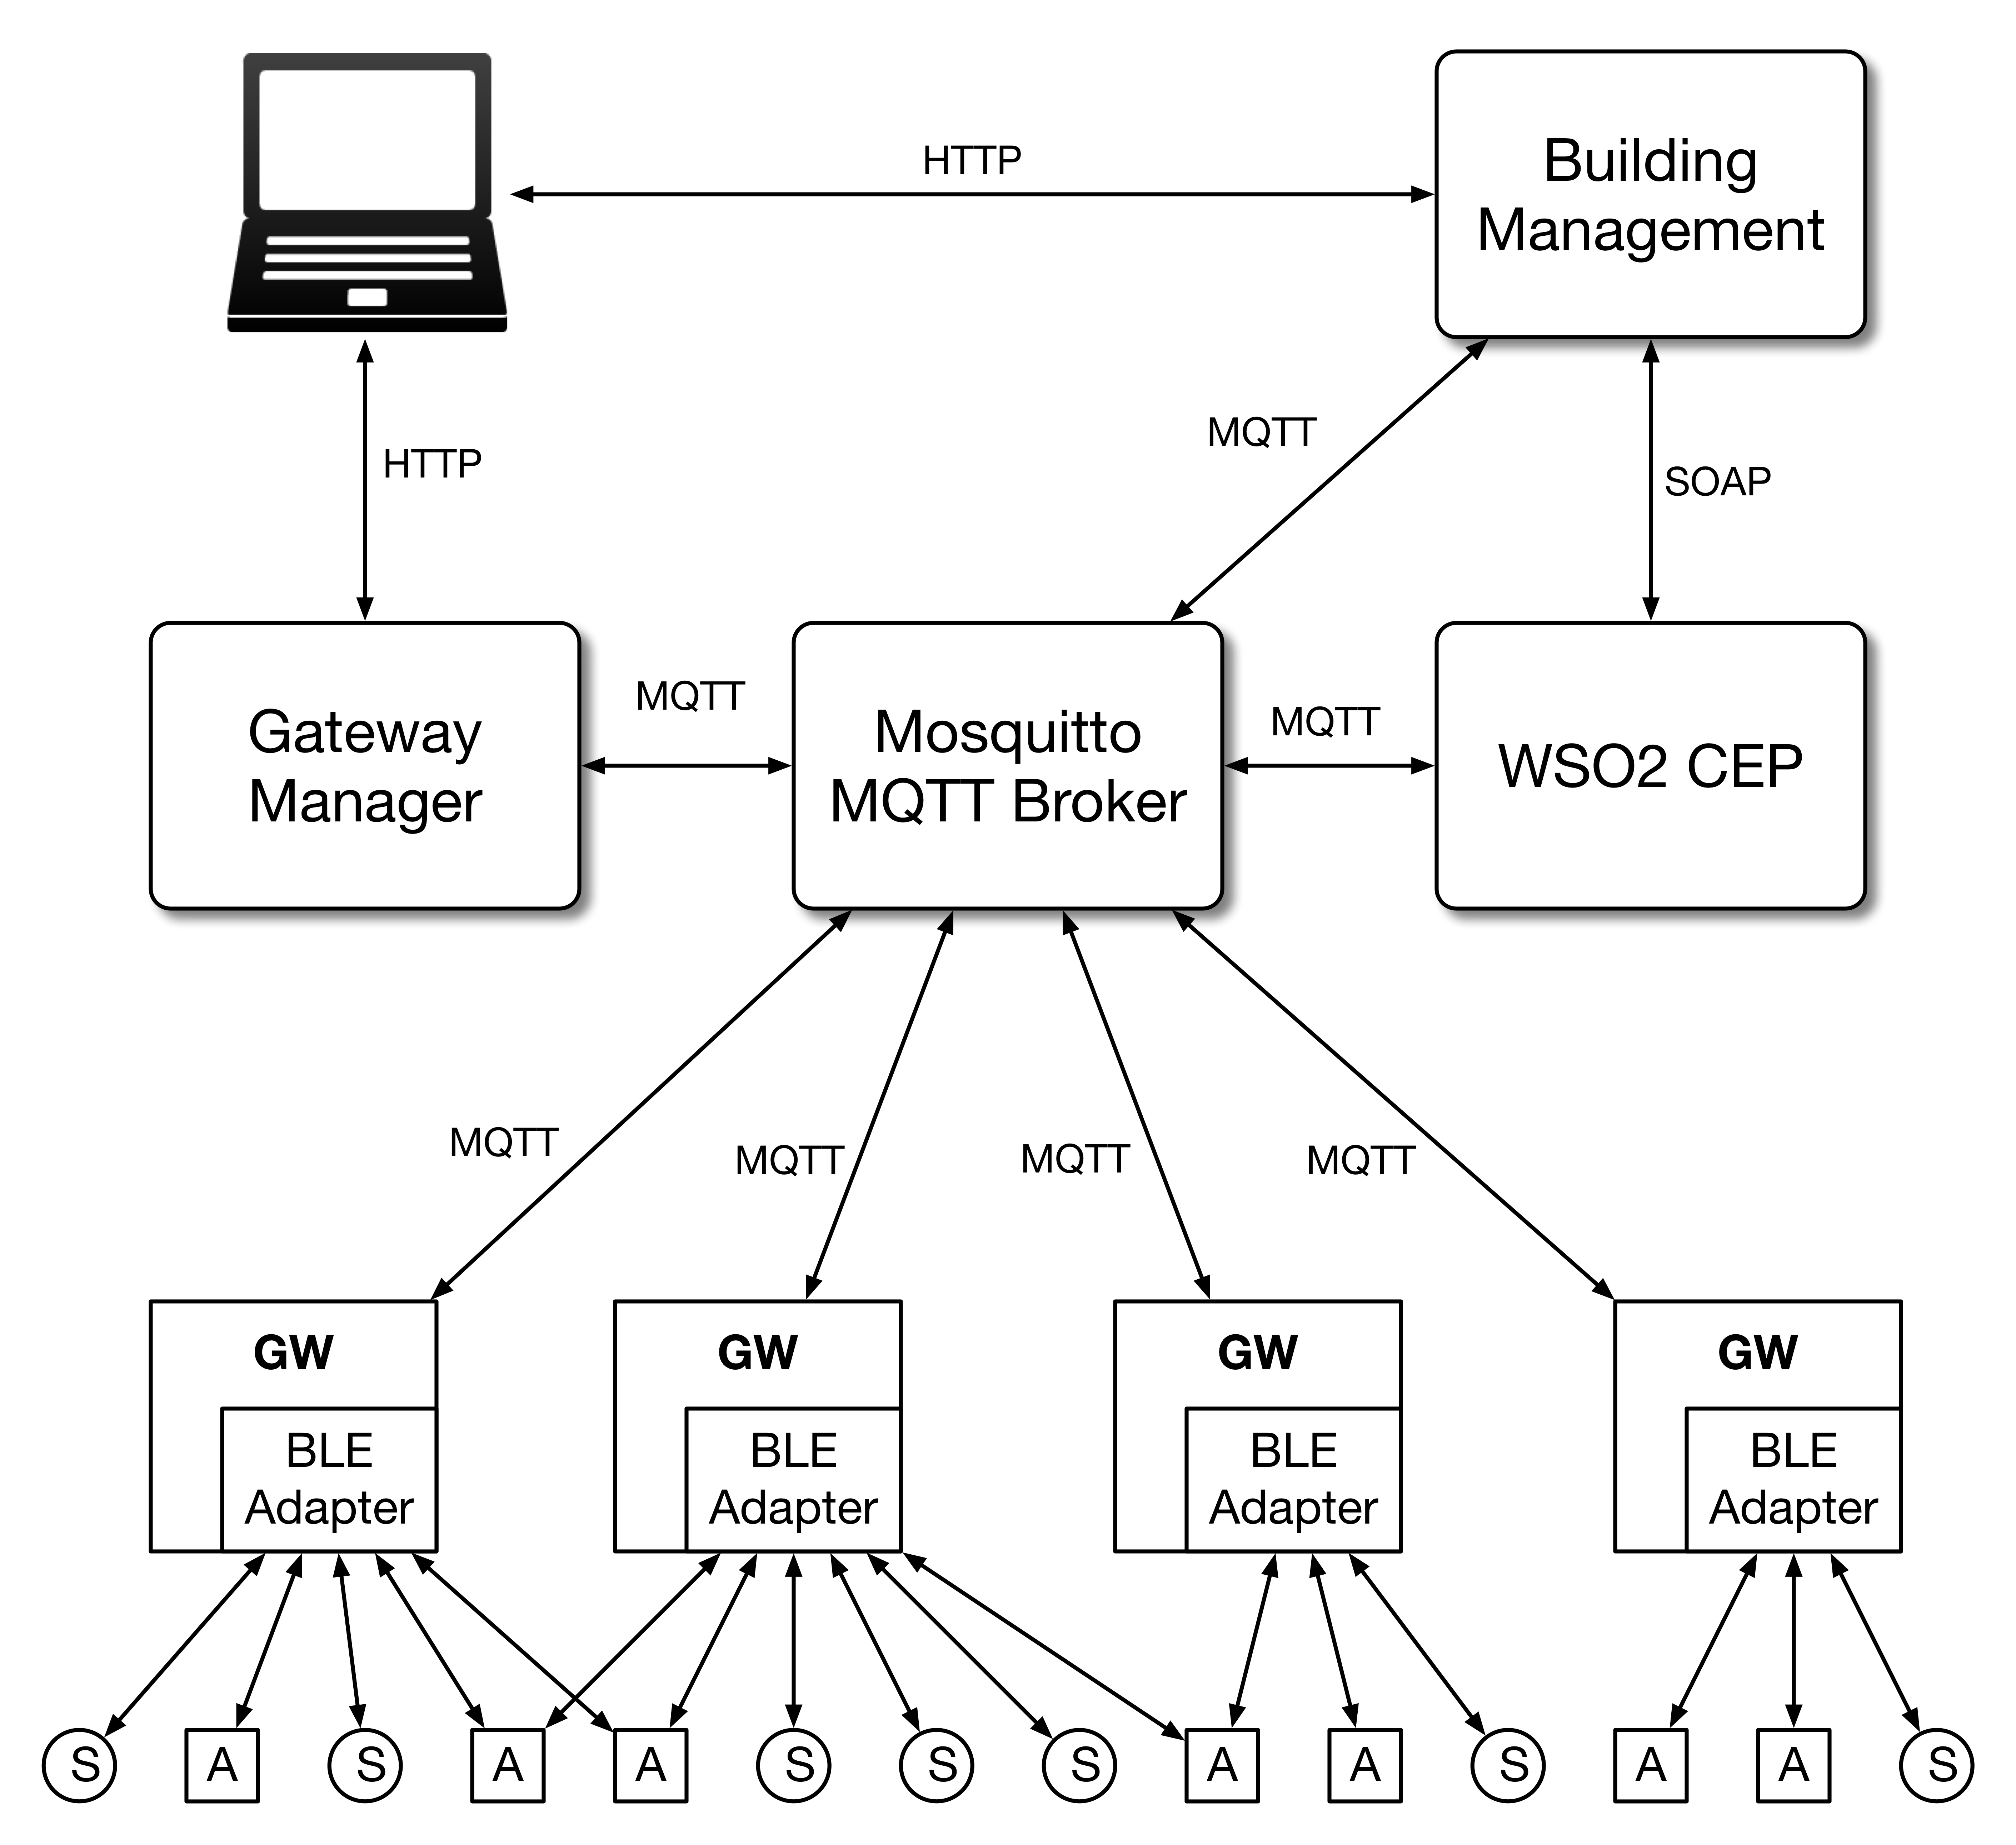
\includegraphics[width=0.9\textwidth]{figures/architecture3.png}
	\caption{Implementation Architecture}
	\label{fig:arch2}
\end{figure}

\subsection{Gateway Manager}
\label{arch:gm}

This section will describe how the Gateway Manager fits in the fulfilment of the requirements and objectives proposed for this project, and also how its features were thought and implemented. 


This component was programmed using Python 3\footnote{https://docs.python.org/3/} and since MQTT was the chosen protocol to communicate with other nodes, the Eclipse Paho MQTT Python client\footnote{https://pypi.python.org/pypi/paho-mqtt/1.3.0} library was used. This client enables the application to connect to a MQTT broker in order to publish messages and subscribe to topics.


\begin{Paragraph}{Rule Parser}
	
One of the Gateway's Manager roles is to receive rules, developed in the existing Building Manager platform 
	


\begin{listing}[H]
	\begin{minted}[
	frame=single
	]{json}
{
 "name": "CorridorsRule",
 "subrules": [{
  "actions": [{
   "target": {
    "type": "mqtt",
    "topic": "/out_events/IT2/Floor0/Corredor/0_13_6/4/all/1501/all/15011/all",
    "value_type": "int"
   },
   "function": {
    "name": "set_value",
    "listen_data": {
     "type": "single",
     "listeners": [{
      "type": "mqtt",
      "topic": "/in_events/IT2/Floor0/Corredor/0_13_6/4/+/3302/+/5500/+",
      "value_type": "int"
     }],
     "window": {
      "type": "time",
      "value": 5,
      "units": "seconds"
     },
     "aggregator": {
      "type": "any"
     }
    }
   }
  }]
 }

\end{minted}
\caption{Example of a simplified message for an event sent to a device.}
\label{snippet:rule}
\end{listing}

\end{Paragraph}

\begin{Paragraph}{System Awareness}

\end{Paragraph}

\begin{Paragraph}{Devices Configuration}

\end{Paragraph}

\begin{Paragraph}{Gateways Configuration}

\end{Paragraph}

\begin{Paragraph}{Building Manager Dashboard}

\end{Paragraph}

\subsection{Gateway}
\label{arch:gw}
TODO

\subsubsection{Automation Rules Definition}
\label{arch:rules}
TODO

\section{Fail Scenarios}
\label{implementation:scenarios}
TODO


